\subsection{Rendering}
\label{sec:rendering-strategy}
% strategies for rendering large amounts of data without storing it on the client computer
The visualisation of large amounts of data becomes problematic when processing the data consumes all of the computational resources of a non-specialised system. 
This is because the resource requirements for processing increase with the size of the data-sets~\cite{Shneiderman2008}. 
Visualisations of large data cubes can still be produced by systems with specialised hardware, but these systems are often limited by their connection to a single geographical location and restricts the number of users able to access the system at a given point in time.
% yanG2017 every line has a source in this bloody paper - refer for more sources
% visualisation is essential to make sense of the data
Visualisation of data is essential to acquire an understanding of it~\cite{Yang2017}. 
Additionally, making the visualisation interactive increases its effectiveness. 
The addition of interaction increases computational overhead as the dataset being visualised must be rendered for each frame displayed.
Changes in the visualisation's appearance resulting from interactions should be perceived as instantaneous. 
Developing a system for producing interactive visualisations of gigantic datasets in real-time is a challenge because hardware will always be pushed to its limits. 
Waiting for hardware technology to catch up with the size of the datasets is futile, as the datasets also increase in size at a steady rate over time.
The increasing size of the datasets can be attributed to many things, but specifically in astronomy it stems from data-capturing instruments becoming more sensitive and more accurate.
To solve this problem would require a system which can scale consistent performance with the ever-increasing datasets without relying on the brute-force strategy for producing visualisations~\cite{Ali2016}.
In the brute force strategy, every single data point within the dataset is visualised regardless of the size of the dataset.

While visualising the entire dataset produces a highly accurate depiction of the data, the amount of time it takes to produce the visualisation is directly linked to the computational power of the hardware.
It could potentially take a long period of time to produce the visualisation if the visualisation is produced on lower-powered hardware~\cite{Fisher2012}.
The length of time can be affected by hardware issues such as system bandwidth, which depends on factors such as the graphical computations, the speed of the display hardware, and the speed at which information can be passed between components~\cite{Becker1987}.
All of the factors present bottlenecks where system performance is potentially stunted.

The rendering speed of the visualisation is crucial to user experience~\cite{MacKenzie1993}, especially in the context of VR, where if the time between updates takes too long it could cause simulator sickness in the user, making the system unusable from the user's perspective. % look for simulator sickness source
For devices with lower-powered hardware to be able to process and visualise the data without negatively affecting system performance the dataset must be reduced in size to reduce the amount of time required to produce a visualisation.
Either through breaking the dataset up into smaller pieces~\cite{Masiane2019, Li2016} or using some sort of data reduction technique to reduce the overall resolution of the dataset through downsampling techniques such as filtering, clustering and sampling~\cite{Masiane2019, Glueck2014}. 

There are problems with both of these approaches.
Dividing the data cube into subsections has the potential to affect the integrity of the data and obscure the context of a section within the larger dataset \cite{Abidi2017}. 
Downsampled data does attempt to preserve as much detail as possible \cite{Dumitrescu2019}, although the integrity of the data cube is affected and some data can be lost.
If the time reduction provided by downsampling the data obscures potential insights, the visualisation becomes useless.
Both of these techniques reduce the accuracy of the visualisation.

The accuracy with which the visualisation is depicted in is incredibly important to the analysis of the data, as discussed further in Section \ref{sec:visual-analytics}.
It is advantageous to give the user a high-level overview of the data at the start if their workflow\cite{Li2016, Lowe2020, Zhao2017}.
This overview can be a downsampled version of the data, which would reduce the processing time because there is less data to be visualised overall\cite{Masiane2019}.
The user must be able to dig deeper into certain areas of interest in order to explore the dataset and uncover insights.
In the architecture of the astronomy visualisation system i-Davie \cite{Marchetti2020}, the user is initially presented with a downsampled version of a data cube and can then explore smaller sections at higher levels of resolution.
i-Davie was made for the exploration of data cubes on a VR device, but the majority of the computation is performed on a co-located computer, typically with mid-range computational power and a GPU.
The i-Davie system workflow is as follows, the user explores the initial data cube and finds an area of interest they would like to explore further.
The user selects that area and crops the section.
i-Davie fetches the higher-resolution version of the selected portion of the data cube.
The user sees these intermediate results at the early stage of the data processing, which allows them to do further exploration based on current knowledge.
This method of progressive visualisation facilitates the exploration of large data cubes.
It allows for speedy access to a visualisation and minimises processing time~\cite{Zhao2017} while also maintaining the accuracy and integrity of the data \cite{Masiane2019}.
% The user sees partial results at the early stage of the data processing and allows them to do further exploration based on a current view to extract knowledge from the data \cite{Zhao2017}.
This method provides required data on demand but does not overwhelm the user with too much information at once.
Even if it is a subsection of the larger data cube the context of the piece of data is understood.
The user understands how that particular section relates to the whole data cube.
This rendering strategy supports the user workflow~\cite{Hassan2011},
initially presenting the user with the full-resolution visualisation does not have a significant improvement to knowledge extraction as, the level of detail visible on the display is limited by the display's resolution. 
The visualisation wastes computational resources by attempting to render points which corresponds to an area smaller than a pixel on the chosen display hardware.
% --------------------------------------------------------------------% what is remote rendering
\subsubsection{Remote Rendering}
The remote rendering strategy is an approach to rendering which offloads computational overhead from lower-powered hardware, such as a laptop or personal computer, to higher-powered hardware, such as a dedicated server.
It makes use of the client-server model;
the server component stores the large data-sets and performs the computationally expensive processes,
whereas the client provides input as requests to the server and displays the output of these requests to the user.
This makes it possible to produce visualisations of datasets which are larger than the client's resources can accommodate~\cite{Hassan2011}.
For remote rendering to function as intended, the client must be able to access any portion of the dataset, and the server and client systems must coordinate with each other to render and display the visualisations in real time~\cite{Glueck2014}.
There are also bottlenecks present in this approach that must be considered.
% network is the biggest bottleneck - want to minimise the overall amount of data sent from server to client as well as the client to the server
The largest bottleneck is the amount of data than can be sent through a network channel in a period of time~\cite{Abidi2017}.
To mitigate the bottleneck the amount of data transferred between the server and client systems needs to be minimised.
% compression is the most common method for counteracting this bottleneck
Compression is the most common method for reducing the bottleneck.
However, compression and decompression consumes CPU on both the client and the server systems and adds time to the rendering process.
It also presents the added chance of losing data during the compression-decompression process.
The system would use lossy or lossless compression, depending on the type of data and how important the integrity of the data is to the functionality of the system.

There are two rendering strategies present in remote rendering; server-side and client side rendering, both of which are prevalent in web application development.
Systems choosing an appropriate approach for their system architecture must consider which strategy would compliment the functionality of the system ~\cite{Iskandar2020}.
% comparison between client-side and server-side rendering in web development
% software architecture
%   choose the right architecture pattern to use to maximise/optimise the utilisation in the given context the application will be used
%   different architectural patterns
%       layered, client-server, master-slave, pipe-filter, broker, peer-to-peer, event-bus, model-view-controller(layered), blackboard, interpreter
% server-side - better search engine optimisation
% client side - better user experience

\paragraph{Client-side Rendering}
% request, download bundle, extract bundle being the web application
In client-side rendering, data is downloaded from a server and then rendered in the client browser.
More specifically, in a web application a request is made to a server, a bundle of data is downloaded.
Once the bundle reaches the web application it extracts the data from the bundle and uses the data in application.
These types of applications use API calls or WebSocket connections to request a from servers.
The process of rendering of volumetric data is the same, data is stored on the server, the data is bundled and sent to the client, the data is extracted and then rendered to produce a visualisation on the client system.
% reduces latency but affects/reduces accuracy
This reduces processing time by rendering the data on the client system.
The compression and decompression of the data during the transfer process can affect its accuracy.
The integrity of the data could also be affected by the downsampling process it went through on the server..
The amount of data that can be rendered is limited to the computational power of the client system while the client system performs other tasks besides those related to the rendering of the data visualisation~\cite{Becker1987}.
In a comparison between client-side and server-side rendering, client-side produces a better user experience~\cite{Iskandar2020}, as the interactions performed on the client are perceived as instantaneous.

\begin{figure*}
    \centering
    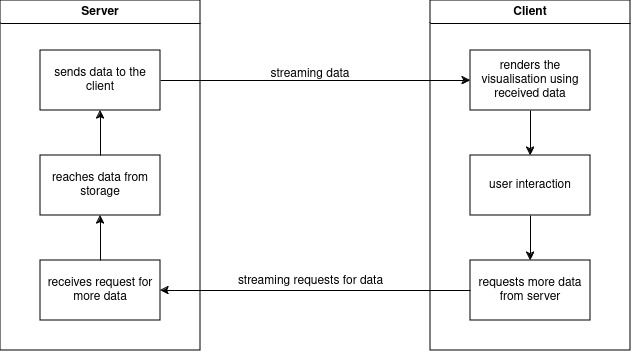
\includegraphics[width=0.6\linewidth]{figures/client-side-rendering.jpg}
    \caption{An example of the process of client-side rendering where data is sent from the server to the client to be rendered. The user interacts with the data on the client and only requests more data from the server when it is required.}
    \label{fig:client-rendering}
\end{figure*}

\paragraph{Server-side Rendering}
% Server side rendering is were static or semi-static web-pages are hosted on a server, and when the user opens a websites these pages are sent from the server.
Server-side rendering involves storing the data on the server and also rendering the data into a visualisation on the server.
Frames of this visualisation are sent to be displayed on the client web application.
% server handles requests from the client, performas actions, and returns a response
The client system has no part in the rendering process, it just displays the frames it receives from the server. 
The user can manipulate the visualisation by forwarding input capture by the client application to the server, following the classic request-response model for web applications.
% In remote visualization (or remote computation) heavy graphics tasks are delegated to a high-end graphics server that actually performs the 3-D rendering and generates a 2-D frame that can be visualized on a remote device (possibly characterized by limited hardware resources). 
The server renders the three-dimensional visualisation of the data but streams two-dimensional images to the client.
% Server-side rendering is implemented when there are computationally expensive graphics tasks that need to be performed.
% These tasks are delegated to the server which has enough computational resources to perform them, whereas the client system does not have the hardware resources to produce the visualisation~\cite{Becker1987}.
% increases accuracy but increases latency 
This strategy increases the accuracy as the integrity of the data is unaffected as it is not processed or transferred, however, it does increase processing time.
The main point where this processing time becomes apparent is when the user performs interactions with a visualisation on the client system.
The user must wait for the interaction to be forwarded to the server, then the visualisation must be re-rendered, and finally the updated frames are streamed to the client.
The time in which these tasks are done increases if the frames are also compressed for transfer over a network, and subsequently decompressed on the client.
The speed of the network the frames are streamed on also affects the processing time of the feedback to the user on the client system.
The slower the network, the more time the user has to spend waiting for feedback.
The server could also have a delayed response because it is performing other tasks, and handling many clients' requests~\cite{Becker1987}.

\begin{figure*}
    \centering
    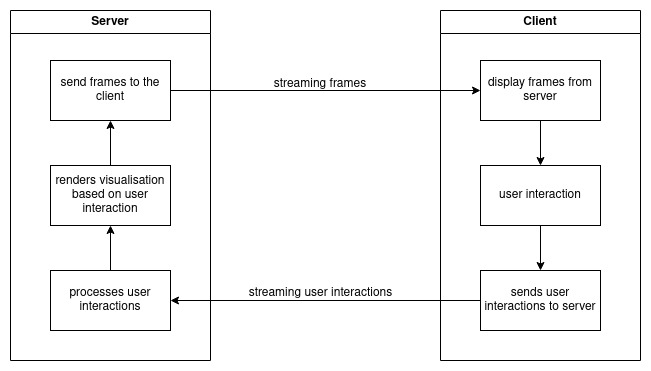
\includegraphics[width=0.6\linewidth]{figures/server-side-rendering.jpg}
    \caption{An example of the server-side rendering process, where the rendering of the data is done on the server and the frames are streamed to the client. The user interacts with the visualisation on the client but the interactions are sent to the server. The rendering is updated based on the user interactions and the frames are once again streamed to the client.}
    \label{fig:server-rendering}
\end{figure*}